\subsection{How is the concept of monitoring implemented in Ambari and Chukwa?}
\label{subsec:Implementation}

\subsubsection{Ambari}
\amb is an open source framework that allows the User to monitore, manage and install Hadoop. It has the abilitie to start, stop and configuratet Hadoop processes automaticly on clusters, without any intervination of the user.\amb was founded to simplifie the use of Hoodop. \cite{Sako2013}
\\
\amb is divided in two parts. First the \amb Web which is the main platform for Users to log in and give up request that should be run through \amb. Secondly the \amb Server, which is divided into smaller parts itself. The API or REST API is connected to different Web applications, the most important one of this is \amb Web. Other interfaces like Microsoft System Center, are applications that allows the user to analyse the data furthermore the capability of Hadoop. The results of the analyse is accessible through \amb Web.
\\
The connection between \amb and Hadoop is done by the \amb Agents. Amabri Server installs on each cluster an \amb Agent, that gives every few seconds a heartbeat to the server; the server answers with an instruction for the Agent or it sends a confermation about his current lifestatus. 
\\
\begin{figure}
\centering
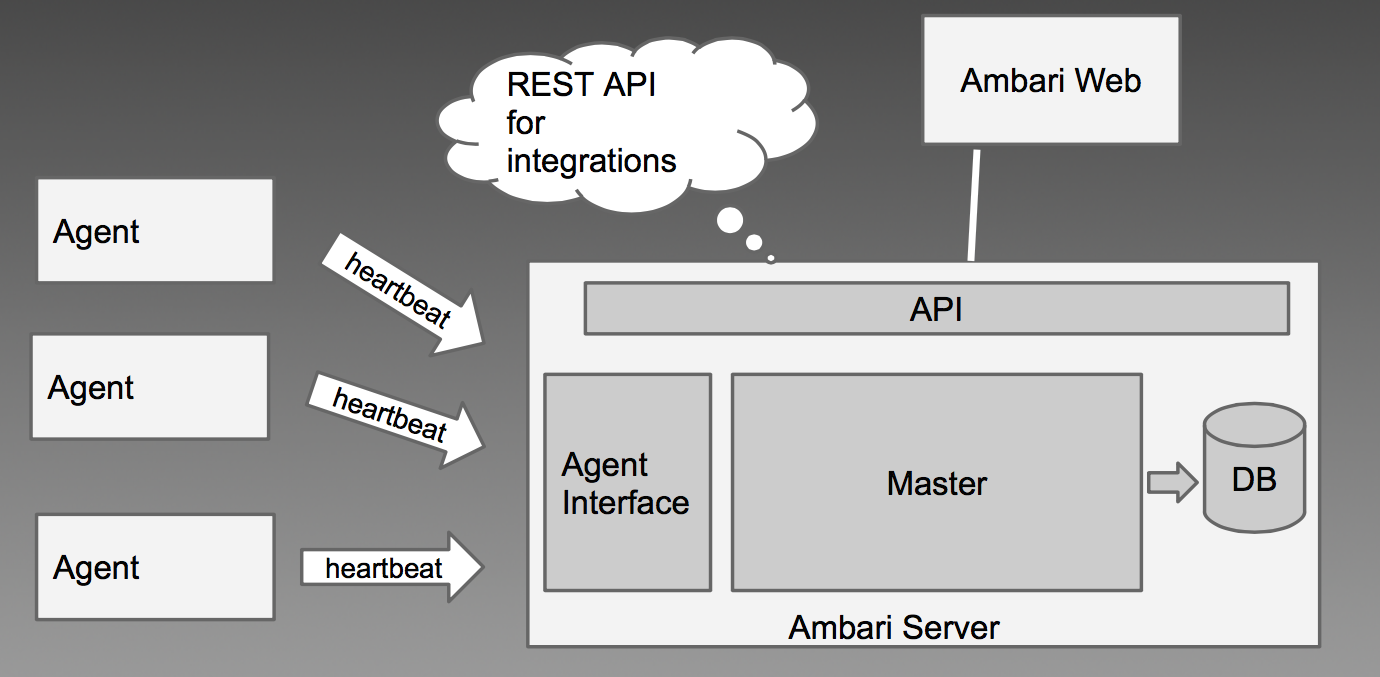
\includegraphics[width=0.7\linewidth]{images/Bild}
\caption{}
\label{fig:Bild}
\end{figure}

The concept of monitoring is given in two spezific ways with \amb\. \amb has the knowling about any cluster healt and its data. It can provide and improve the health situation of a Hadoop cluster and analyse the data in ways there are usefull for the user. The user has an overview on the current siruation through the Web application. \amb divieds to monitroing Prozess in three parts. The first one is the List of all the Application Amabari is running on any of the connected Clusters. It shows the name, status und number of clusters that are in defoult, and need to get be fixed. The second part is explain all the technical details about the application, such as storing space and running time. The last part is aimed to show illustrativly how long and effective an application has been running on any clusters. Based on this data the user can give up requests to change the applications or add more clusters into one process, through the API. \amb then will install automaticly an new application to the cluster on sending heartbeat information to the \amb Agent. 

\subsubsection{Chukwa}
\chuklong is ``a data collection system for monitoring and analyzing large distributed systems.''~\cite{Boulona}
It is build to support log handling on scalable Hadoop clusters. Chukwa is developed at Yahoo!~\cite{Rabkin2008a}